\documentclass[
  digital,
  oneside,
  nosansbold,
  nocolorbold,
  lof,
  lot
]{fithesis4}

\usepackage[resetfonts]{cmap}
\usepackage[T1]{fontenc}
\usepackage[
  main=english,
  english, german, czech, slovak
]{babel}

\usepackage{paratype}

\thesissetup{
    date        = \the\year/\the\month/\the\day,
    university  = mu,
    faculty     = fi,
    type        = bc,
    department  = Department of Computer Science,
    author      = Petr Kubica,
    gender      = m,
    advisor     = {RNDr. Jan Mrázek.},
    title       = {Jaculus: Approachable Programming of Embedded Devices via Javascript},
    TeXtitle    = {Jaculus: Approachable Programming of Embedded Devices via Javascript},
    keywords    = {keyword1, keyword2, ...},
    TeXkeywords = {keyword1, keyword2, \ldots},
    abstract    = {
      This is the abstract of my thesis, which can

      span multiple paragraphs.
    },
    thanks      = {
      These are the acknowledgements for my thesis, which can

      span multiple paragraphs.
    },
    bib         = bibliography.bib,
    facultyLogo = fithesis-fi,
}
\usepackage{makeidx}
\makeindex
\usepackage{paralist}
\usepackage{url}
\usepackage{markdown}
% \def\markdownRendererCodeSpan#1{\colorbox{gray!10}{#1}}
\usepackage{listings}
\lstset{
  basicstyle       = \footnotesize\ttfamily,
  identifierstyle  = \color{black},
  keywordstyle     = \color{blue},
  keywordstyle     = {[2]\color{cyan}},
  keywordstyle     = {[3]\color{olive}},
  stringstyle      = \color{red},
  commentstyle     = \itshape\color{teal},
  breaklines       = true,
  showstringspaces = false,
  % backgroundcolor  = \color{gray!10},
}
\usepackage{floatrow}
\floatsetup[table]{capposition=top}
\usepackage[babel]{csquotes}


\lstdefinelanguage{js}{
  keywords={typeof, new, true, false, catch, function, return, null, catch, switch, var, if, in, while, do, else, case, break},
  ndkeywords={class, export, boolean, throw, implements, import, this},
  comment=[l]{//},
  morecomment=[s]{/*}{*/},
  morestring=[b]',
  morestring=[b]",
}

\lstdefinelanguage{cpp}{
  keywords={alignas, alignof, and, and_eq, asm, atomic_cancel, atomic_commit, atomic_noexcept, auto, bitand, bitor, bool, break, case, catch, char, char8_t, char16_t, char32_t, class, compl, concept, const, consteval, constexpr, constinit, const_cast, continue, co_await, co_return, co_yield, decltype, default, delete, do, double, dynamic_cast, else, enum, explicit, export, extern, false, float, for, friend, goto, if, inline, int, long, mutable, namespace, new, noexcept, not, not_eq, nullptr, operator, or, or_eq, private, protected, public, reflexpr, register, reinterpret_cast, requires, return, short, signed, sizeof, static, static_assert, static_cast, struct, switch, synchronized, template, this, thread_local, throw, true, try, typedef, typeid, typename, union, unsigned, using, virtual, void, volatile, wchar_t, while, xor, xor_eq},
  comment=[l]{//},
  morecomment=[s]{/*}{*/},
  morecomment=[l][\color{violet}]{\#},
  morestring=[b]',
  morestring=[b]",
}


\begin{document}

\shorthandoff{'}
\begin{markdown*}{%
  hybrid,
  definitionLists,
  footnotes,
  inlineFootnotes,
  hashEnumerators,
  fencedCode,
  citations,
  citationNbsps,
  pipeTables,
  tableCaptions,
}

\chapter{Motivation}

Microcontrollers in embedded devices are typically programmed in compiled languages, such as C, C++, or Rust. Although these languages provide high performance and low overhead at runtime, they can be difficult to learn and use.

Another problem of compiled languages in embedded environments is a long development cycle. Because of the limited resources of a microcontroller, the executable of such applications is usually self-contained, and, besides the application itself, contains all used libraries, including the standard ones. All of the libraries must be linked on every build and in some cases also compiled regardless of whether they have changed. The development cycle is often further prolonged by long deployment times. The build-deploy process can take several minutes, severely hindering development speed, especially in the early development stages when the developer rapidly iterates over the code.

Teaching embedded programming to beginners is a big motivator for reducing the development cycle length. Seeing the results of their work quickly is important for keeping them motivated and interested in the subject, especially with children and their increasingly short attention span.

As embedded devices often interact with the physical world or communicate with other devices, they often have to wait for external events rather than actively perform some computation. Therefore, most embedded applications have reactive and asynchronous elements, which are difficult to express in low-level languages. This induces a lot of boilerplate code, which obfuscates the main application logic and makes it harder to develop and maintain. Even though high-level languages such as C++ and Rust somewhat alleviate this issue, C is often the only language with direct support from the manufacturers, adding more work for the developer.


\chapter{Proposed solution}

The proposed solution is to use a high-level, interpreted language instead. The language has to:

  - have low enough hardware requirements to run on a microcontroller
  - be easy to learn and use
  - be able to express reactive and asynchronous elements
  - be embeddable into C/C++ applications

The solution should also provide an ecosystem for managing the device and developing applications. The ecosystem should include:

  - a firmware for the microcontroller, which gives complete control over the device to the runtime environment and provides an API for managing the device
  - a command-line application for managing the device and uploading code to it

\section{Language choice}

Many interpreted languages are available. Because of their popularity in embedding into other applications, the following languages were considered:

  - Python
  - Lua
  - JavaScript

Python is a general-purpose language with an extensive standard library, which makes it suitable for many applications. However, it is not suitable for embedded platforms due to its high memory requirements caused by its large standard library.

Lua is a lightweight scripting language with a small standard library. It is suitable for embedded devices and there are Lua interpreters, which are embeddable into C/C++ applications. On the other hand, Lua is not nearly as popular as Python and JavaScript, making it harder to find relevant resources and justify learning a new language.

JavaScript is a popular language commonly used in web browsers. The language specification defines a small standard library, which is extended by the runtime environment, meaning a small memory footprint. It also maps very well to the event-centered nature of many embedded systems, as JavaScript is inherently event-driven. Multiple embeddable JavaScript engines exist, such as DukTape, MuJS, and QuickJS.

For the above reasons, JavaScript was chosen to be used in the final solution.

Because JavaScript is weakly typed, debugging errors caused by type mismatches is sometimes challenging. A possible solution is to use a strongly typed language, such as TypeScript. However, as compiling or running TypeScript on a microcontroller is not feasible, it must first be transpiled\footnote{Transpilation refers to the process of source-to-source compilation} to JavaScript.


\chapter{Overview}

The main task is to create a JavaScript runtime environment for microcontrollers and an ecosystem around it for managing the device and developing applications for it.

The runtime should primarily focus on the ESP32 and ESP32-S3 microcontrollers, as they are prevalent in the maker community and provide high performance at a low price.

A firmware for a microcontroller, which gives complete control over the device to the JavaScript runtime and provides an interface for programming and controlling the device, should be created. A device running this firmware will be called a *Jaculus device*.

\section{Runtime environment}

The runtime environment should be able to run JavaScript code and be easily extensible with functionality implemented in C++. The runtime should be usable as the main interface for programming the device and as a component of a larger application.

An example use case for the latter is in a system of devices used as game elements. Their low-level logic (e.g., communication, user interface) can be implemented in C++, while the high-level logic (e.g., game rules) can be updated independently by the user.

\section{JavaScript engine}

A JavaScript engine is needed to interpret JavaScript code. Implementing a custom JavaScript engine would be a significant undertaking, so an existing one is used instead. There are multiple options, the popular ones being V8, DukTape, MuJS, QuickJS.

The V8 engine is the most popular JavaScript engine, used in Google Chrome and Node.js. It is a high-performance engine with a very large memory footprint, making it impossible to run on a microcontroller.

DukTape and MuJS are small, embeddable JavaScript engines. They are suitable for embedded devices but support old versions of the ECMAScript specification.

QuickJS is a small, embeddable JavaScript engine that supports the ECMAScript 2020 specification. On a desktop platform, it is 2-4 times faster\cite{quickjs} than DukTape and MuJS, for the price of a larger memory footprint, which is still small enough to run on a microcontroller.

The final solution uses QuickJS. Compared to the other options, it stands on a nice middle ground regarding its feature set, performance, and memory footprint.

\section{Communication}

There should be a way to communicate with the device --- to upload code, control the runtime and monitor the device's state.

Most microcontrollers feature a serial interface, such as a USB to UART bridge or a native USB interface. A serial interface, however, only provides a single duplex byte stream, meaning a protocol must be implemented on top of it to enable communication with multiple services over a single connection.

Using a single stream connection also adds flexibility in the choice of the transport medium. Aside from the serial interface, the protocol can be used over a network socket, web socket, or any other byte stream connection.

\section{Tooling}

A suitable tooling should be created to support the development of applications for the device. The tools should allow the user to upload code to the device, control the runtime, and monitor the device's state.

\section{Implementation}

To achieve the goals described above and to allow possible future reuse of independent components, the project is split into multiple parts:

  - Jaculus-machine -- standalone, embeddable, C++ centric JavaScript runtime using QuickJS at its core
  - Jaculus-link -- standalone communication library for multiplexing multiple channels on a single stream connection
  - Jaculus-dcore -- core library for creating new Jaculus devices
  - Jaculus-tools -- command-line application for controlling and monitoring Jaculus devices
  - Jaculus-esp32 -- Jaculus device port for the ESP32 platform (with support for ESP32 and ESP32-S3 SOCs)


\chapter{Used technologies}

This chapter briefly describes some selected technologies used in the project and some of their specifics.

\section{ESP32 and ESP32-S3}

ESP32 and ESP32-S3 are microcontrollers by Espressif Systems.

ESP32 is a dual-core microcontroller based on the Xtensa LX6 CPU architecture with 520 KiB of SRAM. It features a UART interface for programming.

ESP32-S3 is a dual-core microcontroller based on the Xtensa LX7 CPU architecture with 512 KiB of SRAM. It features a native USB interface and a UART interface for programming.

Both of these microcontrollers also provide a Wi-Fi and Bluetooth interface and a large number of other peripherals. On many boards based on these microcontrollers, the programming UART interface is connected to a USB-to-UART bridge, which allows the microcontroller to be programmed over USB. The USB ports are also often used for communication with the program running on the microcontroller.

\section{ESP-IDF}

ESP-IDF is the official development framework for microcontrollers from Espressif Systems. The framework is based on FreeRTOS and provides a set of libraries and tools for developing applications for, besides others, ESP32 and ESP32-S3 microcontrollers.

Most of the provided libraries have only a C API. The framework also supports C++20 with a large subset of its standard library. However, some parts of the standard library do not work entirely correctly (e.g., `std::filesystem`).

\section{JavaScript}

JavaScript is a high-level, interpreted, weakly, and dynamically typed programming language. It is standardized in the ECMAScript specification, which is maintained by Ecma International.

Although JavaScript programs are event-driven, the code is executed in a single thread. This is achieved by using an event loop, where asynchronous events are queued and executed in the order they are received. Therefore, JavaScript programs must be written in a non-blocking manner, as blocking the event loop will cause the program to stop responding to events. Events are generated by the JavaScript engine or the host environment both synchronously and asynchronously.

\section{TypeScript}

TypeScript is a strongly typed superset of JavaScript. It is developed and maintained by Microsoft. TypeScript is typically not interpreted directly and is instead compiled into JavaScript, which can be interpreted using any JavaScript runtime that supports the specified ECMAScript version.

\section{QuickJS}

QuickJS\cite{quickjs} is a JavaScript engine implementing the ECMAScript 2020 specification\cite{es2020} (ES2020). It was developed by Fabrice Bellard and is licensed under the MIT license. It is written in C and is designed to be embeddable in other applications.

QuickJS uses POSIX to implement atomic operations and system time. Although this slightly limits its portability, ESP-IDF, the primary target platform for Jaculus, supports POSIX.

According to ES2020, JavaScript code is evaluated in a *Realm*, which defines the execution environment (e.g., global object and set of built-in objects). QuickJS uses a different term for this concept --- Context, which I have adopted for Jaculus and will be used throughout the rest of this thesis.


\shorthandon{'}
\end{markdown*}


\shorthandoff{'}
\begin{markdown*}{%
  hybrid,
  definitionLists,
  footnotes,
  inlineFootnotes,
  hashEnumerators,
  fencedCode,
  citations,
  citationNbsps,
  pipeTables,
  tableCaptions,
}

\chapter{Jaculus-machine} \label{chap:machine}

Jaculus-machine is a standalone, embeddable, C++ centric JavaScript runtime. It uses the QuickJS JavaScript engine at its core and provides a set of C++ classes that wrap the QuickJS API. The main goal of Jaculus-machine is to provide a simple and easy-to-use API for adding features to the runtime.

A large portion of Jaculus-machine is a set of wrapper classes around the QuickJS API. The classes provide RAII semantics and an easy-to-use API for routine use cases.

Jaculus-machine uses two core concepts, which will be referred to as *Machine* and *MFeature* throughout the rest of this thesis.

  - Machine --- an instance of the runtime complete with all the selected MFeatures
  - MFeature --- a component that can be used as a part of a Machine and which provides functionality to the runtime or to other MFeatures

((TODO: proc modularni))

\section{Design}

The main entry point of the library is a Machine object. After a Machine is created and initialized, it can be used to interact with the JavaScript runtime and execute JavaScript code.

((TODO: why wrapper, more about wrapper))

\subsection{Machine and MFeatures}

A Machine is defined using templated stack inheritance from `MachineBase` and selected MFeature classes. The `MachineBase` class provides the core functionality of the runtime, and the MFeature classes implement additional functionality, such as an event loop and filesystem access.

The stack design of the Machine allows interfacing with different MFeatures in C++ directly without any middleware. Lower-level MFeatures are located lower in the stack and implement platform-specific functionality, while higher-level MFeatures are located higher in the stack and can use the abstraction provided by the lower-level MFeatures. This allows for easy portability of higher-level MFeatures to other platforms.

\subsection{Exceptions}

A portion of the Jaculus-machine library consists of wrappers that allow calling C++ functions from JavaScript code. When an exception is thrown in the wrapped C++ code, it is caught by the wrapper, converted to a JavaScript exception, and propagated to the runtime. The library allows the user to specify the JavaScript `Error` type or any other JavaScript value that should be thrown.

Similarly, when a JavaScript function is called from C++, and an exception is thrown in the runtime, it is caught by its wrapper, converted to a C++ exception of type `jac::Exception`, and propagated to the C++ code.


\section{Features}

Jaculus-machine mainly consists of wrappers around QuickJS API. The wrappers provide RAII semantics and an easy-to-use API for routine use cases.

The library provides a minimum set of MFeatures that are required for the runtime to function correctly or are helpful for development and debugging. Instead, the library aims to provide functionality, which makes the creation of new MFeatures as easy as possible.


\subsection{Value wrapping}

QuickJS uses reference counting for memory management, and the user is responsible for decreasing the reference count of JavaScript values that are no longer needed. Jaculus-machine provides a set of classes that wrap JavaScript values and provide RAII semantics for them. The classes also provide a simple API for converting to and from C++ types.

The base class for JavaScript value wrapper is `ValueWrapper` and provides a general API for working with JavaScript values. More specific wrapper classes are derived from `ValueWrapper` and provide additional functionality, such as `ObjectWrapper` and `FunctionWrapper`.

The wrapped value can be either a value (e.g., a number) or a reference (e.g., an object).
`ValueWrapper` has a template parameter `managed` that defines whether the wrapper takes ownership of the underlying JavaScript value. This pattern is assumed from QuickJS, which sometimes does not give ownership of the value to the user to reduce the number of changes in its reference count. If the value is a reference, depending on the value of `managed`, the wrapper will either be a strong or a weak reference to the value. For convenience, the library provides two type aliases for all built-in wrappers, which are usually used instead and follow the following pattern:

```cpp
// value/strong reference
using Value = ValueWrapper<true>;
// value/weak reference
using ValueWeak = ValueWrapper<false>;
```

\subsection{Type conversions}

In many cases, the library can perform automatic type conversions between JavaScript values and C++ types. Among others, automatic conversions happen in getters, setters, and function calls. This allows for wrapping existing functions without having to write conversion code manually.

Default conversions for several built-in types are provided, such as `int`, `double`, `std::string`, and `std::vector`. The library also provides a mechanism for defining custom conversions for user-defined (and not-yet-supported built-in) types.

\subsection{Function wrapping} \label{sub:func-wrapping}

The library provides an interface for defining JavaScript functions by wrapping most existing callable C++ objects. This interface is presented in the form of `FunctionFactory` class.

Because variadic functions in C++ are processed at build time, they can not be universally wrapped to create their JavaScript counterparts. For this reason, `FunctionFactory` lets the user define a function with an argument of type `std::vector<ValueWrapper>`. When this function is called from JavaScript, the vector will contain all arguments passed to the function.

The created wrappers then automatically perform argument and return type conversions and convert any exceptions thrown by the wrapped function to a JavaScript exception.

\subsection{Class wrapping} \label{sub:class-wrapping}

((TODO: example))
Sometimes, it is desirable to create a JavaScript object backed by a C++ object. This can be done using the class `Class`. The class is templated by a `ProtoBuilder` structure, which defines how the JavaScript object prototype should be constructed and how the optional opaque data should be managed. The class `Class` can then be used to initialize the class in a given Context, construct the JavaScript object or obtain its constructor.

\subsection{Built-in MFeatures}

The following MFeatures are included with the library (their class names are suffixed with "Feature" in the library):

  - EventQueue -- an asynchronous event queue that can be used to schedule events to be executed in the event loop; the events can be scheduled from any thread
  - EventLoop -- an event loop that executes events from an event queue in the main thread
  - Filesystem -- an abstraction over the filesystem that provides access to files and directories
  - ModuleLoader -- an implementation of module loader for loading modules from the filesystem (using the `import` statement in JavaScript) and evaluating JavaScript files (using the `evalFile` method in C++)
  - BasicStream -- an implementation of simple readable and writable stream types
  - Stdio -- a feature adding `stdin`, `stdout`, and `stderr` streams to the Machine and `console` interface only to the runtime
  - Timers -- typical JavaScript timers and a sleep function

\subsection{Watchdog}

The `MachineBase` class provides a watchdog timer that can be used to detect infinite loops in the runtime. The watchdog can be configured using the `setWatchdogTimeout` method. By setting the timeout to 0, the watchdog can be disabled. It is disabled by default.

By default, the watchdog will interrupt the runtime on timeout. This behavior can be changed by setting the watchdog handler using the `setWatchdogHandler` method. Instead of interrupting, the handler will be called, and depending on its return value, the runtime will either be interrupted or continue running.


\section{Implementation}

The library is implemented using C++20 and requires POSIX for QuickJS.

All public functionality is contained in the `jac` namespace. QuickJS exports its symbols in the global namespace, and their names are usually prefixed with `JS`. The user should not interact with QuickJS directly for regular use, as the library provides wrappers for most of its functionality.

\subsection{Default event loop}

Default event loop implementation is split into two separate MFeatures. One implements an event queue, and the other implements the event loop. This allows for easier portability, as the event loop itself can be reused on different platforms, while the event queue can be extended to, for example, support scheduling events from interrupts.


\section{Usage} \label{sec:machine-usage}

The central part of the library is the `Machine` type, which represents a JavaScript runtime with a set of MFeatures. An example definition of a Machine is shown below:

```cpp
using Machine = ComposeMachine<
    ModuleLoaderFeature,
    FilesystemFeature,
    StdioFeature,
    BasicStreamFeature,
    MachineBase
>;
```

The `ComposeMachine` class is a helper class that builds the Machine inheritance chain. The MFeatures at the beginning of the argument list will be at the top of the stack, and the MFeatures at the end will be at the bottom. The `MachineBase` class is a base class for all Machines and must be at the end of the list.

\subsection{Adding the library to a project}

((TODO))

The library is configured as a CMake project. It exports a CMake target called `jac-machine` that can be linked to other projects.

\subsection{JavaScript values}

The `ValueWrapper` class represents JavaScript values, which can be obtained either as a result of the execution of JavaScript code or by wrapping a C++ value. New JavaScript values can be created using static methods of the `ValueWrapper` and its subclasses. The following code shows some examples:

```cpp
ContextRef ctx = ...;

Value undefined = Value::undefined(ctx);
Value number = Value::from<int>(ctx, 42);
Value string = Value::from<std::string>(ctx, "Hello, world!");
Value object = Object::create(ctx);
Value array = Array::create(ctx);
```

The `ValueWrapper` class provides methods for converting the wrapped value to a C++ value:

```cpp
Value value = ...;

int number = value.to<int>();
std::string string = value.to<std::string>();
```

If the wrapped value cannot be converted to the requested type, a `jac::Exception` will be thrown.

\subsection{JavaScript exceptions}

Wrapped C++ code can throw exceptions. If that happens, the wrappers will catch the exception, convert it to a JavaScript exception, and throw it to the JavaScript runtime. The following exception types are converted as follows:

  - `jac::Exception` -- the exception is converted to a specified `Error` type, or to the wrapped value if `type == Type::Any`
  - `std::exception` -- the exception is converted to an `InternalError` object with the message `e.what()`
  - any other exception -- the exception is converted to an `InternalError` object with the message "unknown exception"

To create an `Exception` that will be converted to JavaScript as a specified `Error` type, the `Exception::create` method can be used:

```cpp
Exception::create(Exception::Type::TypeError, "invalid argument");
```

To create an `Exception` that will be converted to JavaScript as a specified value, the value should be created independently and then converted to an `Exception` using the `ValueWrapper::to` method:

```cpp
Value value = ...;
Exception exception = value.to<Exception>();
```

\subsection{Wrapping C++ functions}

As described in Section \ref{sub:func-wrapping}, the library provides a mechanism for wrapping callable C++ objects into JavaScript functions through the class `FunctionFactory`.

To wrap a function, the user can use the `newFunction` and `newFunctionThis`. All arguments that are passed to the function call will be converted to the types of the function parameters. If the number of arguments does not match or if the values cannot be converted to the required types, a `TypeError` will be thrown.

The methods `newFunctionVariadic` and `newFunctionThisVariadic` can be used to create variadic functions --- all arguments that are passed to the function call will be contained in a single `std::vector<ValueWeak>`.

The methods `newFunctionThis` and `newFunctionThisVariadic` additionally give access to the `this` value of the function (for example, when the function is called as a method of an object).

The following code shows some examples:

```cpp
ContextRef ctx = ...;
FunctionFactory ff(ctx);

Function add = ff.newFunction([](int a, int b) { return a + b; });

Function sum = ff.newFunctionVariadic([](std::vector<ValueWeak> args) {
    int sum = 0;
    for (auto& arg : args) {
        sum += arg.to<int>();
    }
    return sum;
});
```

\subsection{JavaScript classes}

As described in Section \ref{sub:class-wrapping}, the library provides a mechanism for creating JavaScript classes, which can be backed by C++ objects.

To create a class, the user must first define a `ProtoBuilder` structure. The `ProtoBuilder` describes the class's behavior and properties through its static interface. Its features are specified by inheriting from the structures in the `ProtoBuilder` namespace and overriding their **static** interfaces. These structs contain a default implementation of their interface and some convenience functions for describing the class. The following code shows an example of a `ProtoBuilder`:

```cpp
struct MyBuilder : public ProtoBuilder::Opaque<MyClass>, public ProtoBuilder::Properties {
  static MyClass* constructOpaque(ContextRef ctx, std::vector<ValueWeak> args) {
    return new MyClass();
  }

  // The default destructOpaque uses delete. By overriding it, we can use a custom deleter

  static void addProperties(ContextRef ctx, Object proto) {
    addPropMember<int, &MyClass::foo>(ctx, proto, "foo");
  }
};
```

The `Class` template can be instantiated with the `ProtoBuilder` structure to create a class definition, and a name can be assigned using the `init` method. The `init` method can be called repeatedly without any effect if called with the same name; otherwise, an exception will be thrown.

```cpp
using MyClassJs = Class<MyBuilder>;
MyClassJs::init("MyClass");
```

To use the class in a given Context, the class must be initialized in the Context by calling the `initContext` method:

```cpp
ContextRef ctx = ...;
MyClassJs::initContext(ctx);
```

After doing the above steps, the user can now get the class constructor and prototype and instantiate the class:

```cpp
Value constructor = MyClassJs::getConstructor(ctx);
Value prototype = MyClassJs::getPrototype(ctx);

Value obj = constructor.to<Function>().callConstructor();
```

\subsection{Creating new Features}

An MFeature is defined as a template class. To allow building the inheritance chain of a Machine, the class must set the class `Next` presented in its last template parameter as its base class. To add functionality to the machine, the class may:

  - present a public C++ interface to MFeatures higher in the inheritance chain or to the user of the Machine
  - use the `initialize` method to add functionality to the JavaScript runtime

In the MFeature constructor, the user must not interact with the JavaScript runtime in any way, as it is not initialized yet. Initialization of the MFeature involving the JavaScript runtime should be done in the `initialize` method.

The following code shows an example of a Feature that adds a `foo` property to the global object:

```cpp
template<typename Next>
class MyFeature : public Next {
    void initialize() {
        ContextRef ctx = this->context();
        Object global = ctx.getGlobalObject();
        global.defineProperty("foo", Value::from(ctx, 42));
    }
};
```

The user might also want to define a JavaScript module. This can be done using the `MachineBase::newModule` method. The following code creates a module named `myModule`, which exports a value named `foo`:

```cpp
template<typename Next>
class MyFeature : public Next {
    void initialize() {
        ContextRef ctx = this->context();

        Module& module = this->newModule("myModule");
        module.addExport("foo", Value::from(ctx, 42));
    }
};
```


\shorthandon{'}
\end{markdown*}


\shorthandoff{'}
\begin{markdown*}{%
  hybrid,
  definitionLists,
  footnotes,
  inlineFootnotes,
  hashEnumerators,
  fencedCode,
  citations,
  citationNbsps,
  pipeTables,
  tableCaptions,
}

\chapter{Jaculus-link}

As described in ((TODO)), the communication between the device and the host is done through a single stream connection.

Because the services running on the device work mostly independently, communicating with each service independently is desirable; this is achieved by multiplexing multiple channels on a single stream connection.

Sometimes, the device may have multiple communication interfaces, which can be used for communication with the host. In such cases, it is desirable to be able to route the communication to the appropriate interface.

This functionality is implemented in the Jaculus-link library, which provides a way to multiplex 256 channels on a single stream connection and to route the communication to the appropriate interface. The library is implemented strictly using only C++ 20 standard library for easy portability. For this reason, it does not provide an implementation for communication interfaces, and the user must provide one themselves.

\section{Architecture}

The model of Jaculus-link is split into three layers:

1. Data link layer
2. Routing layer
3. Communicator layer

\subsection{Data link}

The data link is responsible for transmitting data along with channel identifiers. The data link provided in this library is implemented in the `Mux` class, which multiplexes 256 channels on a single stream connection.

It is possible to use other data link implementations as long as they implement the `DataLinkTx` interface for transmission and provide a way to connect them to a `DataLinkRx` for processing received data.

\subsection{Routing layer}

The routing layer is responsible for routing received data to the consumer of the channel. The routing layer is implemented in the `Router` class.

A `Router` instance can be connected to multiple data links and will route data from all of them to the appropriate consumer with the information about the link it was received from. It also allows sending data to a specific link and channel.

\subsection{Communicator layer}

The communicator layer is used as an abstraction layer for communicating through channels. Typically, the communicator is associated with a single channel and provides either an interface for sending or receiving data.

Communicators used for receiving data from a `Router` must implement the `Consumer` interface, which allows them to be subscribed to a specific channel on a `Router` instance. They must process the received data without blocking, preferably only by storing the data in a buffer and processing it later.

Communicators that send data do not have a unified binding interface. Instead, they access the `Router` instance directly and send data to a specific channel on a specific link (or links).

\subsection{Full Jaculus-link pipeline}

The default configuration of the full pipeline provided by the library is shown in the diagram in Figure \ref{fig:link-pipeline}.

\begin{figure}[!ht]
    \centering
    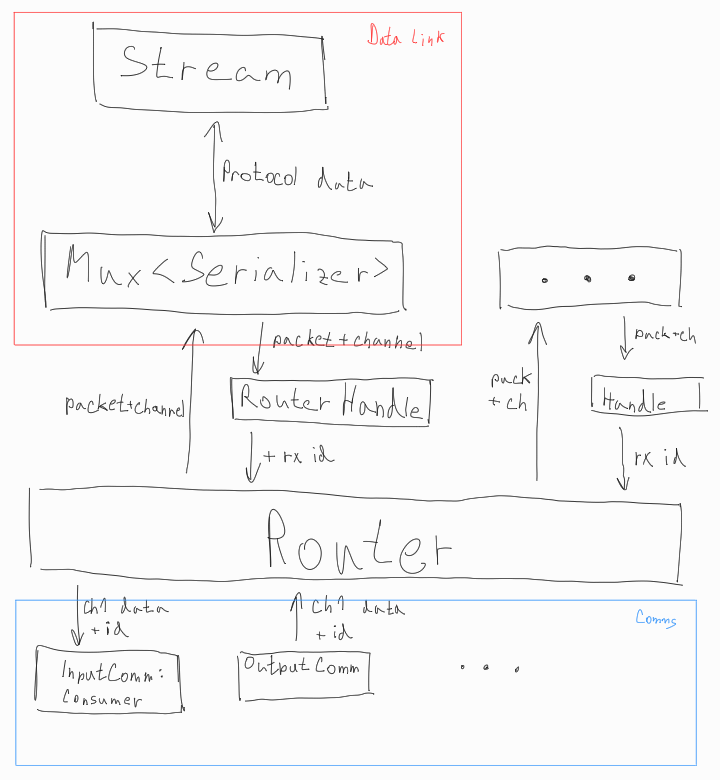
\includegraphics[width=\textwidth]{img/link-pipeline}
    \caption{Default configuration of full Jaculus-link pipeline}
    \label{fig:link-pipeline}
\end{figure}


\section{Multiplexer protocol}

The library provides one protocol for the multiplexer in the class `CobsEncoder`. The protocol is based on a modified version of the COBS\cite{cobs} algorithm for data framing and was originally proposed\footnote{The discussion can be found at \url{https://github.com/yaqwsx/Jaculus/pull/15}.} by Jaroslav Malec for the use in the predecessor version of the Jaculus project.

In the original COBS algorithm, a delimiter byte --- typically zero --- is inserted at the end of the data frame. To encode the transmitted data, every occurrence of the delimiter byte in the data is replaced by a value, that represents the number of bytes to the next delimiter byte. This allows for data framing with a fixed two-byte overhead while limiting the maximum data size to 254 bytes.

The modified version of the algorithm moves the delimiter byte to the start of the data frame and adds length information to the second byte of the data frame. The rest of the data frame is encoded in the same way as in the original algorithm, except for the missing delimiter byte at the end of the data frame, which is only implied by the data frame length. Every such data frame has a three-byte overhead and can contain up to 254 bytes of data. Moving the delimiter byte to the start of the data frame allows for resetting the packetization state in case a previous data frame is lost, malformed, or other corrupted data is received on the stream.

Figure \ref{fig:cobs-diagram} shows a data frame structure diagram. In the data section of the data frame, the first byte contains the channel identifier, followed by the transmitted data. The last two bytes of the data frame contain the CRC16 checksum of the data section.


\begin{figure}[!ht]
    \centering
    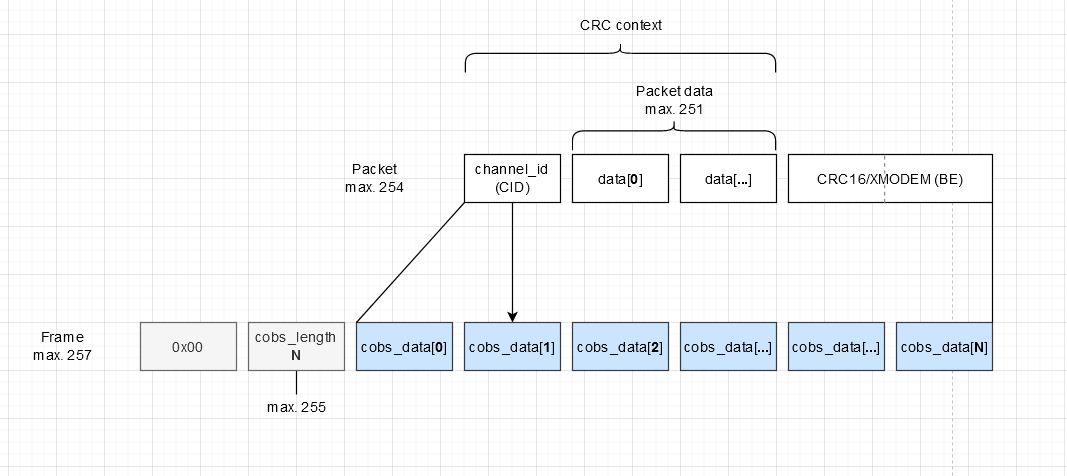
\includegraphics[width=\textwidth]{img/cobs-diagram}
    \caption{Diagram of the COBS-based multiplexer protocol}
    \small{Adapted from: MALEC, Jaroslav. *Protocol diagram*. In: GitHub \[online\]. 2021 \[visited on 2023-05-10\]. Available from: \url{https://github.com/yaqwsx/Jaculus/pull/15}.}
    \label{fig:cobs-diagram}
\end{figure}


\section{Usage}

\subsection{Adding the library to a project}

Jaculus-link is a header-only library, so it is sufficient to add the `include` directory to the include path of the project. The library is also configured as a CMake project and exports a target `jac-link` that can be linked to other projects.

\subsection{Multiplexer}

The class `Mux` is a data link implemented as a multiplexer and is templated on the type of the underlying multiplexer protocol. The only protocol provided with the library is in the `CobsEncoder` class. To implement another protocol, the user can create a class with the same interface as `CobsEncoder`.

The `Mux` constructor takes a `Duplex` instance, which serves as an abstraction around the stream connection.

\subsection{Router}

The `Router` class implements the routing layer.

A `Router` instance can be connected to multiple data links as shown in the following example:

```cpp
// Create a router
Router router;

// Create a stream connection
auto stream = std::make_unique<MyStream>();

// Configure a data link
Mux<CobsEncoder> mux(std::move(stream));

// Connect the data link to the router
auto handle = router.subscribeTx(1, mux);
mux.bindRx(std::make_unique<decltype(handle)>(std::move(handle)));
```

The `handle` object is used to receive data from the data link and must be bound to the same data link instance as the one used to subscribe to the router, as it adds the information about the data link to the received data.

\subsection{Communicators}

The communicators are used as an abstraction layer for communicating through channels. Communicators provide an interface for sending or receiving data through a channel.

The provided communicator types are:

- `OutputStreamCommunicator` --- sends data as a stream of bytes
- `InputStreamCommunicator` --- receives data as a stream of bytes
- `OutputPacketCommunicator` --- sends data while exposing the underlying data framing
- `InputPacketCommunicator` --- receives data while exposing the underlying data framing

These communicator types are only interfaces, and their implementations for `Router` are provided in classes with the same names prefixed with `Router`.

The following example shows how to create a pair of stream communicators:

```cpp
Router router;

// Create an input stream communicator
RouterInputStreamCommunicator input({});

// Subscribe the communicator to the router
router.subscribeChannel(1, input);

// Create an output stream communicator and connect it to the router
RouterOutputStreamCommunicator output(router, 1, {});
```


\shorthandon{'}
\end{markdown*}


\shorthandoff{'}
\begin{markdown*}{%
  hybrid,
  definitionLists,
  footnotes,
  inlineFootnotes,
  hashEnumerators,
  fencedCode,
  citations,
  citationNbsps,
  pipeTables,
  tableCaptions,
}

\chapter{Jaculus-device-core}

The Jaculus-device-core library provides a mechanism for defining a Jaculus device and controlling it.

It uses the Jaculus-machine library for the JavaScript runtime and the Jaculus-link library for communication.

% \section{Features}

%   - Jaculus-machine runtime
%   - communication via Jaculus-link
%   - control protocol for controlling and monitoring Jaculus-machine runtime
%   - uploader protocol for uploading code/data to Jaculus device

\section{Architecture}

\subsection{Device class}

The `jac::Device` class is the entry point for defining a Jaculus device. It is a template parametrized by the Machine type used for the JavaScript runtime. The Machine type must implement the `evalFile` method, which is used to run the code uploaded to the device.

The `jac::Device` class exposes a `jac::Router` object, which is used to connect the device to the communication channel/s. `jac::Device` also exposes an interface for controlling the internal Machine instance from C++ code.

Two services are also part of the `jac::Device` class and expose functionality over the communication channel/s:

  - Uploader - service for uploading code/data to the device
  - Controller - service for controlling and monitoring the device

Each service uses a single channel provided by the `jac::Router` object. Other channels are also reserved for the standard input and output of the Machine instance and for a global logger instance.

The `jac::Device` implements a locking mechanism to prevent multiple clients from accessing the device simultaneously. The lock is paired with a timeout, which is reset while the client communicates with the devices. If the timeout expires, the lock is released, and other clients can access the device. The lock is exposed to the client via the Controller service.


\section{Implementation}

\subsection{Controller service}

The Controller service is implemented in the `jac::Controller` class. It uses a *PacketCommunicator* interface to communicate with the client. The first byte of each packet is used to specify the command to be executed. The rest of the packet is used to transmit command-specific data.

The service provides the following functionality:

  - accessing the device lock
  - controlling the internal Machine instance
  - using the Machine instance's standard input and output
  - monitoring the device status

\subsection{Filesystem access}

The Uploader service provides access to the filesystem of the device. Unfortunately, because `std::filesystem` is not yet fully implemented in ESP-IDF, the implementation has to, in some cases, rely on the POSIX filesystem API to be portable to the ESP platform.

\subsection{Uploader service}

The Uploader service is implemented in the `jac::Uploader` class. Similarly to the Controller service, it uses a *PacketCommunicator* interface to communicate with the client. The first byte of each packet is used to specify the command to be executed. The rest of the packet is used to transmit command-specific data.

The service provides the following functionality:

  - listing files and directories
  - creating and deleting directories
  - writing, reading, and deleting files

Most commands are processed in a single packet, but writing files requires the data to be sent in multiple packets. When writing a file, an internal state is set to specify what operation should be performed when data is received and when the transmission is finished. To prevent overflow of the receiving buffer, the command implements, admittedly relatively inefficient, flow control -- the client must acknowledge each packet before the next one is sent.

Commands for reading a file and listing a directory might also split the data into multiple packets. For simplicity, no flow control is implemented when transmitting data to the client, as the client is expected to be a much more powerful device that can handle the transmission.


\section{Usage}

  - defining a Jaculus device
  - controlling a Jaculus device


\shorthandon{'}
\end{markdown*}

\shorthandoff{'}
\begin{markdown*}{%
  hybrid,
  definitionLists,
  footnotes,
  inlineFootnotes,
  hashEnumerators,
  fencedCode,
  citations,
  citationNbsps,
  pipeTables,
  tableCaptions,
}

\chapter{Jaculus-tools}

To allow the user to interact with Jaculus devices, a command-line application called Jaculus-tools was created. The application is implemented in TypeScript and is available as an npm package under the name `jaculus-tools`.

The package could also be used as a library for building custom applications, but it is not documented. The user might want to look at the source code of the command-line application part of the package for inspiration on how to use the library.

\section{Features}

The application provides commands to check the status of the device (`status`, `version`), install the Jaculus firmware (`install`), control the JavaScript runtime (`start`, `stop`, `monitor`), and access the device's filesystem (`ls`, `read`, `write`, `rm`, `mkdir`, `rmdir`, `upload`). The application also provides commands for uploading and downloading code to the device (`build`, `flash`, `pull`).

Other utility commands are also available:

  - `help` -- prints help for the specified command
  - `list-ports` -- lists available serial ports
  - `serial-socket` -- tunnel a serial port over a TCP socket

The commands are run by specifying them after the `jac` command.

```
$ jac <command> [options] [arguments]
```

\section{Implementation}

\subsection{Connection to the device}

The application implements a simplified version of the interface described in ((TODO - Jaculus-link)) -- the `Router` class is omitted, as connecting to multiple devices is mostly pointless. Aside from that and language choice, the implementation is almost identical.

\subsection{Device access}

The application provides access to the device via the `Device` class. The class exposes the following functionality to the user:

  - device lock
  - Controller and Uploader services
  - standard input and output of the running program
  - output of the device logger

\subsection{Command-line argument parser}

The application uses a custom parser for command-line arguments, which allows for chaining compatible commands.

The commands can also access and modify a global state object passed to each command, allowing them to share data --- for example, once the device is connected, the `Device` instance is saved to the state object and can be accessed by other commands.

For example, the following command:

```
$ jac --port /dev/ttyUSB0 build flash monitor
```

Will sequentially run the three specified commands (`build`, `flash`, `monitor`). The `build` command compiles the code and saves the compiled code to `build` directory. The `flash` command connects to the device, saves the device to the parser state, and uploads the code. The `monitor` command uses the saved device to access its standard input and output without reconnecting.

Command-line options are divided into two types -- global and command-specific. Options can be specified in any place of the command, as the parsing is done in multiple passes for each specified command. The global options are parsed first, then options of the first command are extracted, then of the second, and so on. Each command then receives only its and the global options. This forces the commands to use different names for their options, as otherwise, preceding commands might extract them. For example, the following two commands would be parsed the same way:

```
$ jac --port /dev/ttyUSB0 build flash monitor
$ jac build flash monitor --port /dev/ttyUSB0
```

The commands can also specify standard arguments, which are parsed after the options:

```
$ jac --port /dev/ttyUSB0 read ./code/index.js
```


\subsection{TypeScript code compilation}


\shorthandon{'}
\end{markdown*}


\shorthandoff{'}
\begin{markdown*}{%
  hybrid,
  definitionLists,
  footnotes,
  inlineFootnotes,
  hashEnumerators,
  fencedCode,
  citations,
  citationNbsps,
  pipeTables,
  tableCaptions,
}

\chapter{Jaculus-esp32}

Jaculus-esp32 is a Jaculus device firmware for the ESP32 family of microcontrollers. It is implemented using the ESP-IDF framework and the Jaculus-dcore library.

\section{Features}

Aside from the features provided by Jaculus-dcore, Jaculus-esp32 only provides control over the most basic peripherals, which are:

  - GPIO -- general-purpose input/output pins
  - ADC -- analog-to-digital converter
  - LEDC -- generator of PWM signals
  - Neopixel -- WS2812B smart LED strip

Jaculus-esp32 also implements a specialized event queue based directly on FreeRTOS queues, supporting scheduling events from an interrupt context. This is used in the GPIO feature for generating events on the input signal change.


\section{Usage}

  - flash manually using ESP-IDF
  - flash using Jaculus-tools


\shorthandon{'}
\end{markdown*}


\shorthandoff{'}
\begin{markdown*}{%
  hybrid,
  definitionLists,
  footnotes,
  inlineFootnotes,
  hashEnumerators,
  fencedCode,
  citations,
  citationNbsps,
  pipeTables,
  tableCaptions,
}

\chapter{Limitations}

This chapter describes the limitations of the created components and the Jaculus-esp32 firmware. While the problems described here are not critical, they cause some inconvenience and should be addressed in the future.

\section{Only one Context per Machine instance}

From the beginning, the design of Jaculus-machine was to have only one Context per Machine instance. It seemed not to be a limiting factor and simplified implementation. However, later in development, it started to show it was a wrong decision and proves to be a limiting factor in some cases.

For example, in REPL, all exceptions should be caught and reported to standard output. When starting REPL from a JavaScript program, the main program should crash on unhandled exceptions, whereas the REPL should not. Implementation of this would require REPL and the main program to be executed in separate contexts to distinguish between their behavior regarding exception handling.


\section{Unhandled promise rejections not being reported}

This is a limitation of QuickJS. Although QuickJS does have a mechanism for reporting unhandled promise rejections, it reports some false positives. Consider the following example:

``` js
new Promise((resolve, reject) => {
    console.log("promise");
    reject(null);
}).then(() => {
    console.log("ok");
}).catch(() => {
    console.log("error");
});

console.log("after");
```

The promise is created and immediately rejected. At that moment, the promise does not have a rejection handler, and thus QuickJS reports an unhandled promise rejection. However, the handler is added before the promise goes out of scope and handles the rejection.

Because of the false positives, the mechanism for reporting unhandled promise rejections is disabled in Jaculus-machine.

Fortunately, this is not a problem for well-written code, which correctly handles all possible promise rejections. However, when an unhandled promise rejection occurs, it is not reported, which may lead to errors that are difficult to debug.

To fix this, modifying QuickJS internals would be required, which is outside the scope of this work, but it is an essential consideration for future work.


\section{Filesystem API}

As the Filesystem MFeature is implemented using C++ `std::filesystem` API, which is not yet fully supported by the ESP-IDF, some of its functionality does not work, and some may even block the runtime indefinitely.

The broken functionality involves listing directories --- `readdir` and `rmdir`. Fortunately, working with files works without a problem, which is an essential functionality for loading JavaScript files.

It would be possible to separately reimplement the MFeature to use the POSIX API, but it would make more sense to implement a more complex abstraction layer around the filesystem API, which could be used by other Jaculus components as well. However, that would require a significant amount of work, which is not strictly necessary for the functionality of Jaculus-esp32.

\section{Compatibility with other platforms}

Through implementing all of the created components, I have focused on only using the standard C++20 library. This worked well for development, as all of the functionality could be tested locally on a desktop PC, and later everything could be easily integrated with the ESP-IDF. Unfortunately, after briefly exploring development options of platforms other than ESP32 (STM32, RP2040), I have discovered that the C++20 standard is often not fully supported. Some platforms do not even fully support older standards, such as C++17.

This has dealt a significant blow to the portability of these components, which would have to be partially rewritten to support other platforms. Primarily, an abstraction layer around the filesystem API and asynchronous elements (threads, synchronization primitives) would have to be implemented.


\shorthandon{'}
\end{markdown*}


\shorthandoff{'}
\begin{markdown*}{%
  hybrid,
  definitionLists,
  footnotes,
  inlineFootnotes,
  hashEnumerators,
  fencedCode,
  citations,
  citationNbsps,
  pipeTables,
  tableCaptions,
}


\chapter{Evaluation}

Several requirements were outlined in the introduction. This section evaluates the solution based on those requirements.

Compared to native programs, the solution significantly reduces the development cycle length. While the development cycle of native programs can, in worse cases, take several minutes, with Jaculus, it is reduced to several seconds. The build time shows the most considerable improvement, as no build process is needed for JavaScript programs, and the build time of TypeScript programs is mostly negligible compared to native programs. Deployment is also faster, as only the application code needs to be uploaded to the device, unlike native programs, where the entire firmware partition is often overwritten.

The shortened development cycle naturally comes at a price, that being the performance of JavaScript as an interpreted language. However, the performance is still sufficient for running most application logic. If a performance-sensitive part of the application is identified, it can be reimplemented in C++ and compiled into a native module.

\section{Comparison with other solutions}

There are already existing solutions to programming microcontrollers using JavaScript. While it would be nice to have a detailed comparison of at least some of them, it would overextend the scope of this thesis. However, a brief comparison of Jaculus with other solutions is provided in this section. These solutions were chosen based on their popularity:

- CircuitPython\cite{circuitpython} (fork of MicroPython\cite{micropython})
- NodeMCU\cite{nodemcu} (Lua)
- Espruino\cite{espruino} (JavaScript)
- Moddable SDK\cite{moddable} (JavaScript)

A common point of these solutions is their much larger feature set compared to Jaculus. They have not only much larger hardware and library support but also larger ecosystems and communities. Espruino and CircuitPython provide very convenient development environments.

What sets Jaculus aside from the other solutions is its much higher-level abstraction around different JavaScript concepts. This allows for much easier wrapping of existing libraries and other code to JavaScript modules, meaning that while the hardware support of Jaculus is currently low, adding more features to the runtime is a quick and straightforward task.

\subsection{Non-JavaScript solutions}

Comparing different languages, especially their performance, is a notoriously difficult task, as each language has its own strengths and weaknesses. Therefore, the comparison focuses on the usability of the solutions.

MicroPython and CircuitPython are implementations of Python~3. They are very popular in the maker community and have a large ecosystem of libraries and tools. However, they only support a limited subset of the language, meaning that some Python code cannot be run on them, which could be seen as a disadvantage.

NodeMCU is a Lua interpreter for ESP8266 and ESP32 microcontrollers. On the one hand, it is a well-established project with an existing community. On the other hand, as mentioned in the introduction, Lua is not nearly as popular as the other languages, making it less attractive to new users.

\subsection{JavaScript solutions}

Comparing Jaculus with the other JavaScript solutions is more straightforward, as they all share the same language. Their main difference is their performance, implementation, and tooling.

Espruino is an open-source JavaScript interpreter for microcontrollers. The biggest problem of Espruino is its low performance, which can be seen in the performance comparison below. Espruino also implements only a limited subset of an older version of the ECMAScript standard, meaning some JavaScript code cannot be run on it. Espruino also provides a convenient development environment through its Web IDE, which allows for live code editing and debugging and does not require any additional tools to be installed.

Moddable SDK is another JavaScript runtime for microcontrollers. It is a commercial product but is open-source and free for non-commercial use. Instead of interpreting the JavaScript code on the device, Moddable SDK compiles it into bytecode on the host machine, packs necessary native libraries, and builds a complete firmware image, which is then uploaded to the device. This approach allows for a smaller runtime footprint but causes a slightly longer development cycle and requires much more complex development tools.

The performance of these solutions was compared by running the same benchmarks on the ESP32 microcontroller. Aside from the GPIO benchmark, the benchmarks were taken from the Computer Language Benchmarks Game\cite{bench-game} and slightly modified for each platform to fit the provided API. The GPIO benchmark was created for this comparison and measured the time it takes to toggle a GPIO pin *n* times. The code of the GPIO benchmark for Espruino is shown below. The results of the comparison are shown in Table \ref{tab:performance}.

```js
var pin = 5;
var start = Date.now();
for (var i = 0; i < n; i++) {
  digitalWrite(pin, 1);
  digitalWrite(pin, 0);
}
var end = Date.now();
console.log("Time: " + (end - start));
```

The benchmarks show that Jaculus is significantly faster in computational tasks than Espruino and Moddable SDK. Moddable SDK is faster in the binary-trees benchmark, which is targeted at the creation of new objects and memory allocation. Moddable SDK is also faster in the GPIO benchmark, which may be caused by poorly optimized abstraction used to implement the native module in Jaculus.

The low performance of Espruino can be likely attributed to the fact that internally, Espruino parses the JavaScript code into an abstract syntax tree, which is then directly interpreted, in contrast to the approach used by Jaculus and Moddable SDK, where the code is first compiled into bytecode and then interpreted.


\begin{table}[ht]
  \centering

  | Test                  | Jaculus     | Espruino    | Moddable SDK |
  |-----------------------|------------:|------------:|-------------:|
  | n-body (n=50)         | 36.2        | 4333.1      | 54.4         |
  | fannkuch-redux (n=6)  | 35.6        | 12335.3     | 75.0         |
  | spectral-norm (n=10)  | 48.9        | 10749.9     | 91.4         |
  | binary-trees (n=3)    | 279.3       | 19930.4     | 187.6        |
  | GPIO (n=5000)         | 756.1       | 11720.4     | 54.7         |

  \caption[Performance comparison of Jaculus with other JavaScript solutions]{Performance comparison of Jaculus with other JavaScript solutions. The results are run times in milliseconds, lower is better.}

  \label{tab:performance}
\end{table}


\chapter{Conclusion}

The goal of this thesis was to create an ecosystem for programming embedded devices using JavaScript.

The presented solution consists of Jaculus-dcore library and Jaculus-tools command-line application. The library provides the core functionality of a Jaculus device, and the application provides a way to interact with the device. The Jaculus-dcore library is also integrated into the Jaculus-esp32 firmware, which ports the solution to the ESP32 platform.

Two standalone libraries were also created as part of the solution: Jaculus-link and Jaculus-machine. The former is a communication library, and the latter is an implementation of the JavaScript runtime with easy extensibility. Both libraries are well documented and tested, and can be used independently of the rest of the solution.

Although the solution is in a usable state and, in terms of performance, can compete with other existing solutions, many features are still missing, and some bugs are present. Most importantly, more MFeatures must be implemented for Jaculus to be a viable alternative to other existing solutions. Further improvements can also be made to the upload protocol, which is currently very simple and could have better performance and reliability.

\shorthandon{'}
\end{markdown*}



\chapter{Future work}

  - Web IDE
  - REPL
  - debugger?
  - add more features
  - support more platforms (e.g. STM32, RPi)
  - uploader protocol optimization and stability improvements

\end{document}
